A lot of tools are available on the Internet to create GUI interface such as Qt, WxWidget, GTK+, FLTK, FOX and some others. I couldn't compare all of them so I have decided to focus on Qt, WxWidget GTK+.

\begin{itemize} 
\item Tools Comparison: \\
I looked accross the Internet to get some testimonies about the different tools and I tried to distinguish them following several criteria - see grid below. 
According to these criteria and considering that Qt is highly recommended for beginners, I have finally decided to use Qt for this project.

\begin{figure}[ht]
\centering
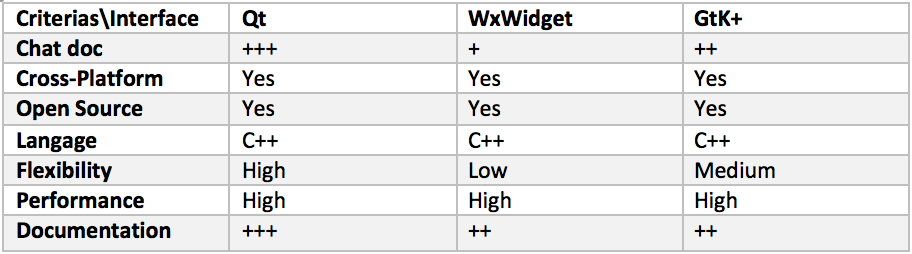
\includegraphics[width = 0.99\hsize]{./figures/comparison}
\caption{LQt, WxWidget, GTK+ comparison table}
\end{figure}
 
\item Qt familiarization: \\
In order to get used to this new tools I have decided to do Openclassroom tutorials [2].
Those tutorials have helped me to install QtCreator and to begin with some basic exercices to get familiar with Qt. I still have some tutorial to do at the current moment but I am feeling comfortable with it.